\documentclass{beamer}
\usetheme{default}

\usepackage{graphicx} % Required for inserting images
\usepackage{geometry}
\usepackage{minted}
\usepackage{hyperref}
\usepackage{mathtools}
\usepackage{enumitem}
\usepackage{amssymb}
\usepackage{float}
\usepackage{caption}
\usepackage{subcaption}
\usepackage[style=ieee]{biblatex}
\setbeamertemplate{bibliography item}{\insertbiblabel}

\DeclareMathOperator{\dom}{\mathbf{dom}}
\DeclareMathOperator{\best}{best}
\DeclareMathOperator{\tr}{\mathbf{tr}}
\DeclareMathOperator{\argmin}{argmin}
\DeclareMathOperator{\sign}{sign}
\let\oldforall\forall
\renewcommand{\forall}{ \, \oldforall \, }

\title{
Subgradient Methods on LASSO Regression
}
\institute{16:332:509}
\author{Kasey Tian}
\date{\today}

\addbibresource{../Report LaTeX/refs.bib}

\begin{document}

\begin{frame}
\titlepage
\end{frame}

\begin{frame}
\frametitle{Outline}
\tableofcontents
\end{frame}

\section{Defining Subgradient}
\begin{frame}
\frametitle{Defining Subgradient}
A subgradient is defined for some convex function \(f: \mathbb{R}^n \rightarrow \mathbb{R}\) at a point \(x \in \dom f\) as a vector \(g \in \mathbb{R}^n\) such that \(\forall y \in \dom f\) \cite{boydvandenberghesubgradient}
\begin{equation}\label{eq:subgradient def}
f(y) \geq f(x) + g^T (y-x) 
\end{equation}
\end{frame}

\begin{frame}
\frametitle{Defining Subdifferential}
There can be multiple subgradients at a point \(x\), so we will also define the subdifferential \(\partial f(x)\) to be the set of all subgradients at \(x\).
\begin{equation}\label{eq:math subdifferential}
\partial f(x) = \bigcap_{y \in \dom f} \left\{ g : f(y) \geq f(x) + g^T (y-x)\right\}
\end{equation}
If there exists at least one subgradient at a point \(x\), we would say \(f\) is subdifferentiable at \(x\). If all points in the domain are subdifferentiable, we say that \(f\) is subdifferentiable. \cite{boydvandenberghesubgradient}
\end{frame}

\begin{frame}
\frametitle{Example: Absolute Value}
\begin{figure}[htbp]
    \centering
    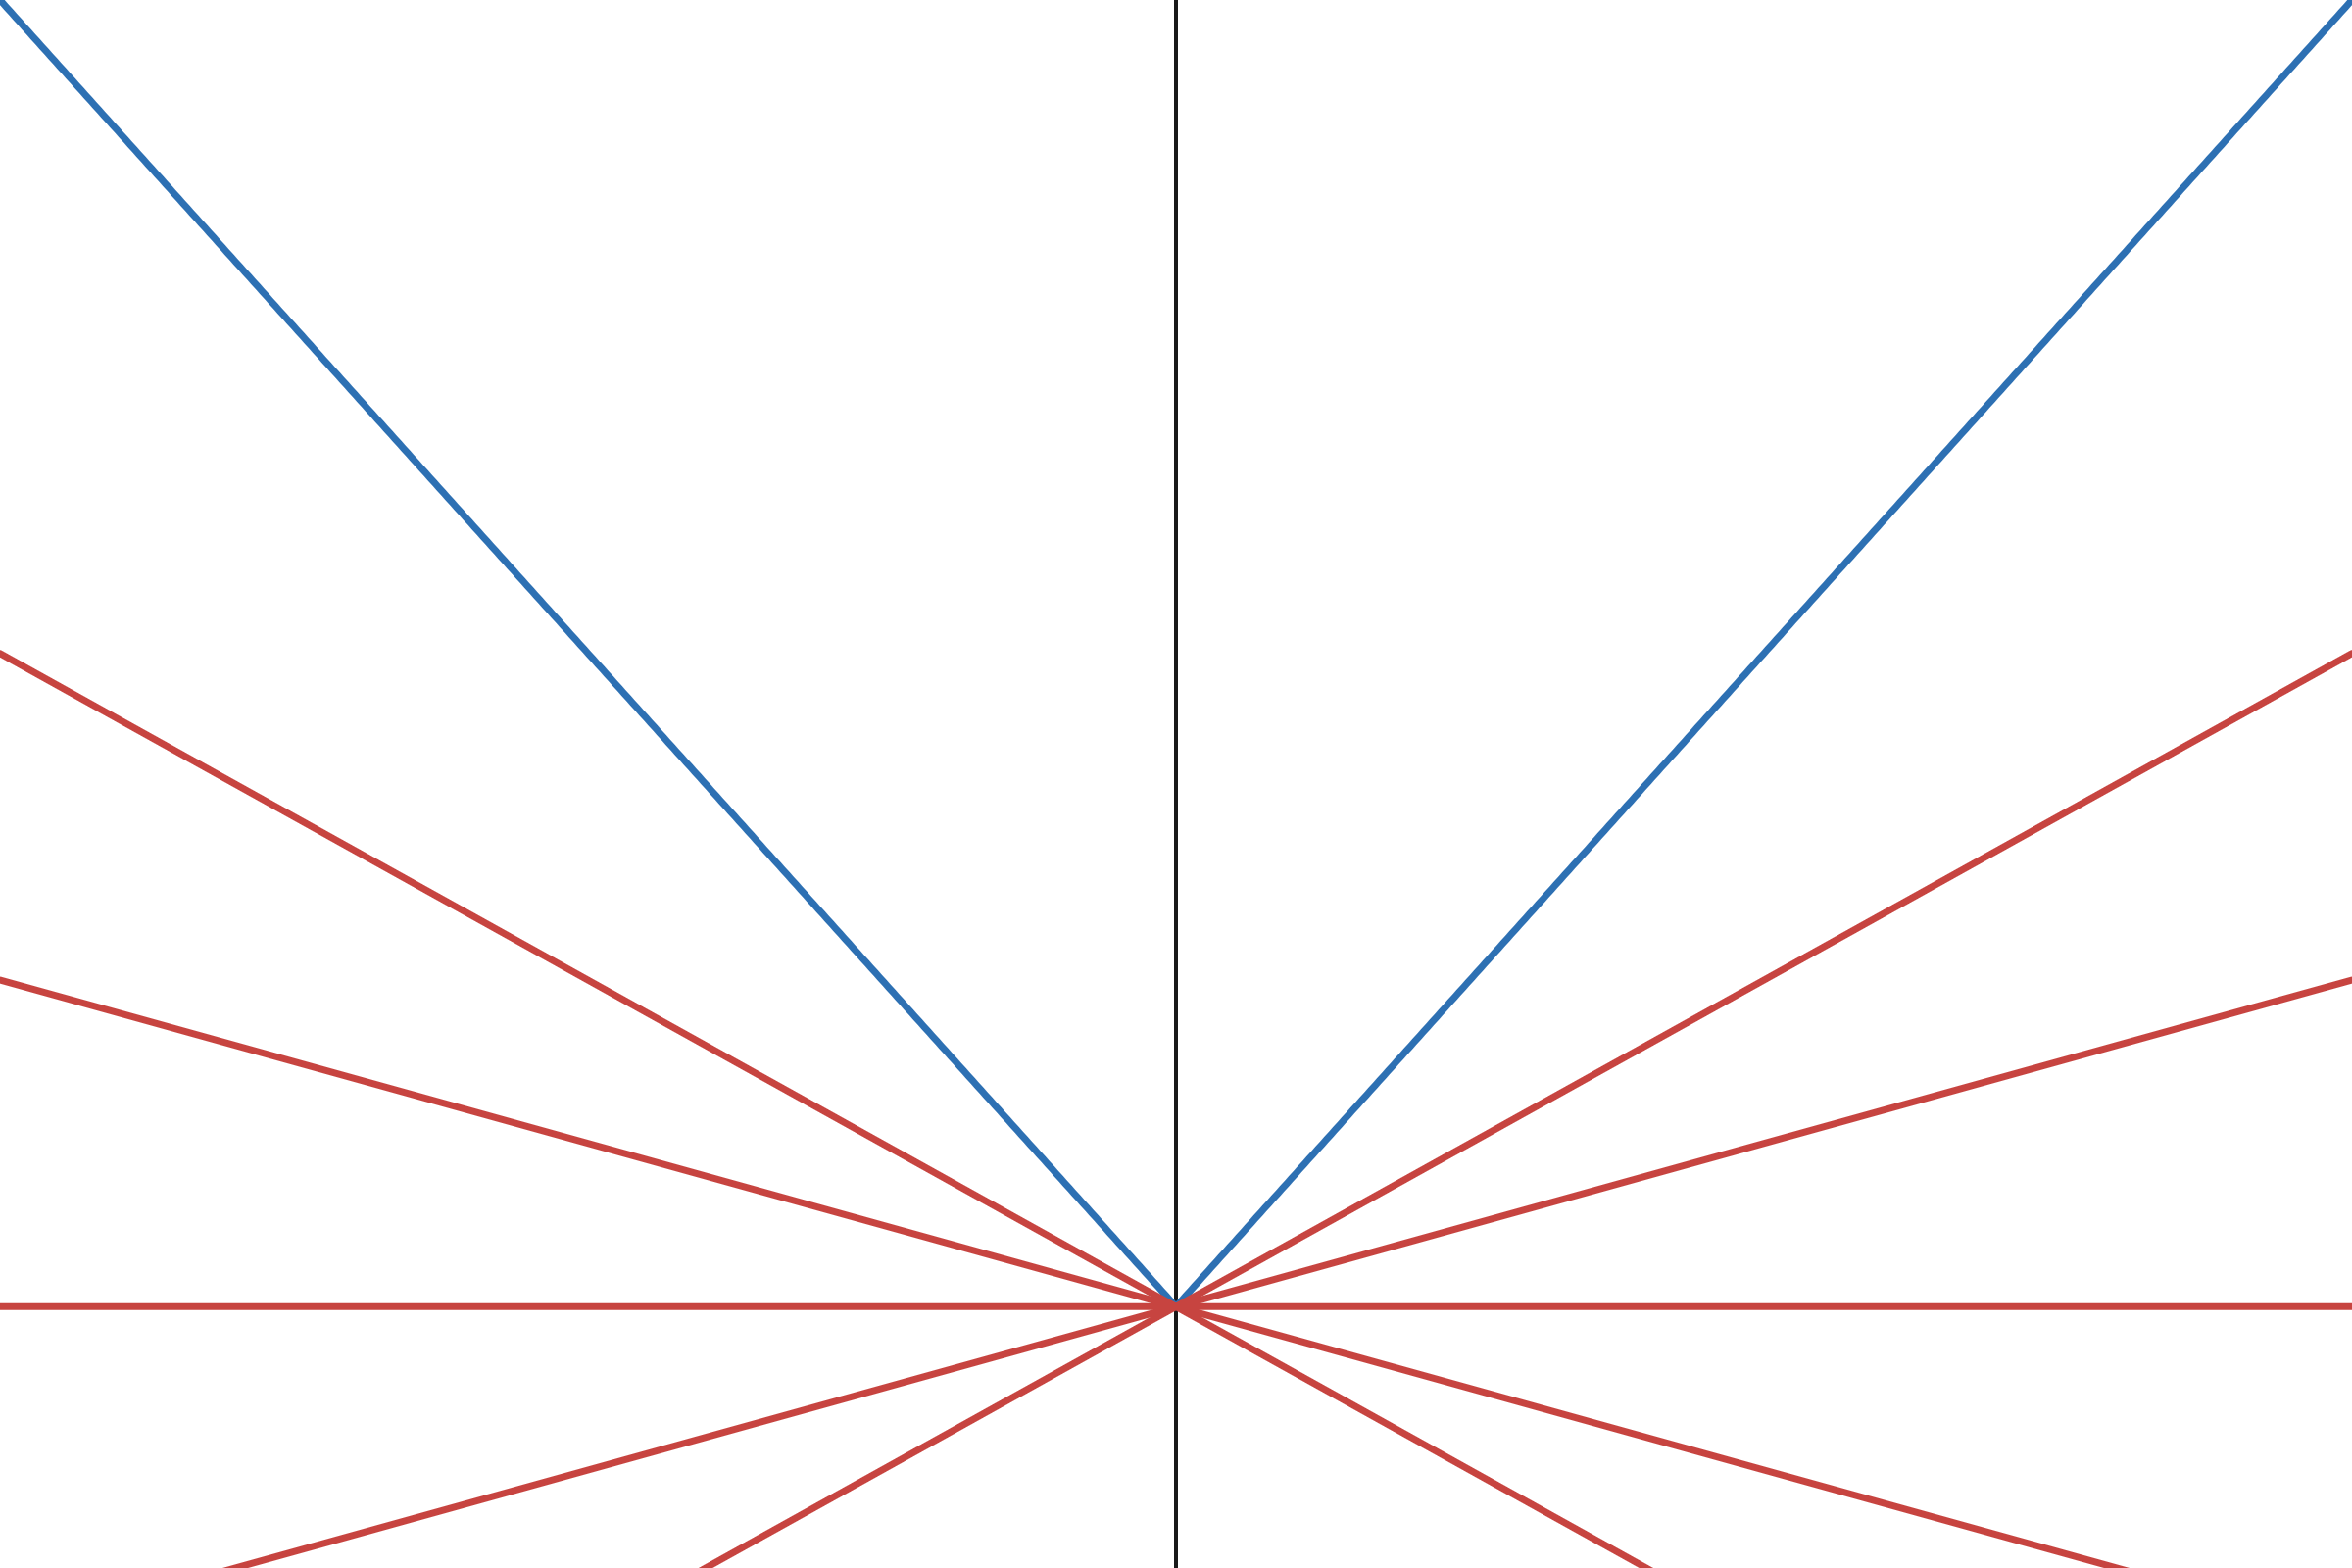
\includegraphics[width=0.5\linewidth]{../Report LaTeX/Figures/abs_subgradients.png}
    \caption{Absolute value function (blue) with subgradients (red)}
    \label{fig:abs subgradients}
\end{figure}
\begin{equation}\label{eq:abs subdifferential}
\partial f(x) = \begin{cases}
    \{-1\} & x < 0 \\
    [-1, 1] & x = 0\\
    \{1\} & x > 0
\end{cases}
\end{equation}
\end{frame}

\section{Subgradient Methods}
\begin{frame}
\frametitle{Subgradient Method Iteration}
Subgradient methods are a family of optimization techniques. They were invented in the 1960s and 70s in the Soviet Union. They all involve the same basic iteration step \cite{boydparksubgradients}
\begin{equation}\label{eq:subgradient method iteration}
x^{(k+1)} = x^{(k)} - \alpha_k g^{(k)}
\end{equation}
where \(g^{(k)}\) is any subgradient at the point \(x^{(k)}\) and \(\alpha_k > 0\)
\end{frame}

\begin{frame}
\frametitle{Subgradient Method Properties}
Subgradient methods are unlike gradient descent and Newton's method in that it is not a descent method. We are not guaranteed that an iteration will descend. Therefore we need to keep track of the best solution we have so far.
\begin{equation}\label{eq:track best}
f^{(k)}_{\best} = \min (f^{(k-1)}_{\best}, f(x^{(k)}))
\end{equation}
And a corresponding \(i^{(k)}_{\best}\) such that \(f(x^{(i^{(k)}_{\best})}) = f^{(k)}_{\best}\)
\end{frame}

\begin{frame}
\frametitle{Subgradient Method Convergence Proof - Assumptions}
\begin{itemize}
    \item There exists a minimizer of \(f\) called \(x^*\), for which \(f^* = f(x^*)\)
    \item There exists some bounding value \(G\) for which \(\|g\|_2 \leq G, \forall g \in \partial f(x), \forall x \in \dom f\)\footnote{One way that this assumption can be met is if the function satisfies the Lipschitz condition, but it is not the only way}\footnote{This assumption helps us greatly in our analysis, but it is not strictly necessary. There exist subgradient methods which can be proven to work even when this assumption does not hold \cite{boydparksubgradients}}
    \item There exists some known bounding value \(R\) such that \(R \geq \|x^{(1)}-x^*\|_2\)
\end{itemize}
\end{frame}

\begin{frame}
\frametitle{Subgradient Method Convergence Proof - Step 1}
\begin{equation}
\begin{aligned}
\|x^{(k+1)}-x^*\|^2_2 &= \|x^{(k)} - \alpha_k g^{(k)}-x^*\|^2_2 \\
\|x^{(k+1)}-x^*\|^2_2 &= \|x^{(k)}-x^*\|^2_2 - 2\alpha_k g^{(k)T}(x^{(k)}-x^*) + \alpha^2_k \|g^{(k)}\|^2_2 \\
\|x^{(k+1)}-x^*\|^2_2 &\leq \|x^{(k)}-x^*\|^2_2 - 2\alpha_k (f(x^{(k)})-f^*) + \alpha^2_k \|g^{(k)}\|^2_2
\end{aligned}
\end{equation}
\end{frame}


\begin{frame}
\frametitle{Subgradient Method Convergence Proof - Step 2}
\begin{equation}
    \begin{aligned}
\|x^{(k+1)}-x^*\|^2_2 & \leq \\ 
    \|x^{(1)} & -x^*\|^2_2 - 2\sum^k_{i=1}\alpha_i (f(x^{(i)})-f^*) + \sum^k_{i=1}\alpha^2_i\|g^{(i)}\|^2_2 \\ 
2\sum^k_{i=1}\alpha_i (f(x^{(i)})-f^*) & \leq R^2  + \sum^k_{i=1}\alpha^2_i\|g^{(i)}\|^2_2 \\
2\sum^k_{i=1}\alpha_i (f^{(k)}_{\best}-f^*) & \leq R^2  + \sum^k_{i=1}\alpha^2_i\|g^{(i)}\|^2_2 \\
f^{(k)}_{\best}-f^* &\leq \frac{R^2  + \sum^k_{i=1}\alpha^2_i\|g^{(i)}\|^2_2}{2\sum^k_{i=1}\alpha_i} \\
f^{(k)}_{\best}-f^* &\leq \frac{R^2  + G^2 \sum^k_{i=1}\alpha^2_i}{2\sum^k_{i=1}\alpha_i}
\end{aligned}
\end{equation}
\end{frame}

\begin{frame}
\frametitle{How to Choose Step Size}
The step size can be chosen in many different ways, we will focus on 5 categories
\begin{itemize}
    \item Constant Step Size
    \item Constant Step Length
    \item Square Summable But Not Summable
    \item Nonsummable Diminishing Step Size
    \item Nonsummable Diminishing Step Length
\end{itemize}
\end{frame}

\begin{frame}
\frametitle{Step Sizes- Constant}
Constant Step Size:
\begin{equation}\label{eq:constant step size}
\begin{aligned}
\alpha_{k} &= \alpha \\
\lim_{k \rightarrow \infty} &\frac{R^2  + G^2 \alpha^2 k}{2\alpha k} = \frac{G^2 \alpha}{2}
\end{aligned}
\end{equation}
Constant Step Length:
\begin{equation}\label{eq:constant step length}
\begin{aligned}
\alpha_k &= \frac{\gamma}{\|g^{(k)}\|_2} \\
\lim_{k \rightarrow \infty} &\frac{R^2  + \gamma^2 k}{2\gamma k / G} = \frac{G \gamma}{2}
\end{aligned}
\end{equation}
\end{frame}

\begin{frame}
\frametitle{Step Sizes - Nonsummable}
Square Summable Not Summable:
\begin{equation}\label{eq:square summable not summable}
\begin{aligned}
\alpha_k &\geq 0 & \|\alpha\|^2_2&= \sum_{k=1}^{\infty} \alpha_k^2 < \infty & \sum_{k=1}^{\infty} \alpha_k &= \infty
\end{aligned}
\end{equation}
Nonsummable Diminishing Step Size:
\begin{equation}\label{eq:nonsummable diminishing step size}
\begin{aligned}
\alpha_k &\geq 0 & 
\lim_{k \rightarrow \infty} \alpha_k &= 0 & 
\sum_{k=1}^{\infty} \alpha_k &= \infty
\end{aligned}
\end{equation}
Nonsummable Diminishing Step Length:
\begin{equation}\label{eq:nonsummable diminishing step length}
\begin{aligned}
\alpha_k &= \frac{\gamma_k}{\|g^{(k)}\|_2} &
\gamma_k &\geq 0 & 
\lim_{k \rightarrow \infty} \gamma_k &= 0 & 
\sum_{k=1}^{\infty} \gamma_k &= \infty
\end{aligned}
\end{equation}
\end{frame}

\section{LASSO Regression}
\begin{frame}
\frametitle{LASSO Regression History}
LASSO is short for \textbf{L}east \textbf{A}bsolute \textbf{S}hrinkage and \textbf{S}election \textbf{O}perator. It was technically first discovered in 1986 by geophysicists, but was later rediscovered, named, and popularized in 1996. It was originally formulated for use with linear classification models, but can be applied to other classifiers as well \cite{lassooriginal} \cite{lassopaper} \\
\end{frame}

\begin{frame}
\frametitle{Problem}
\begin{itemize}
    \item The problem is \(p\) dimensional with a scalar outcome
    \item We analyze \(n\) cases at a time
    \item Collected inputs form the matrix \(X \in \mathbb{R}^{n \times p}\)
    \item Collected outputs form the vector \(y \in \mathbb{R}^n\)
    \item Parameters are \(\alpha \in \mathbb{R}\), \(\beta \in \mathbb{R}^p\)
    \item Our classifier takes the form \(y = \beta^T x + \alpha\)
\end{itemize}
\end{frame}

\begin{frame}
\frametitle{LASSO Estimate}
\begin{equation}\label{eq:lasso estimate}
\begin{aligned}
(\hat{\alpha}, \hat{\beta}) &= \argmin \left\{ \sum_{i=1}^{n} \left(y_i-\alpha-\sum_{j=1}^p \beta_j X_{i,j}\right)^2 \right\} \\
\textrm{s.t.} &\sum^p_{j=1} |\beta_j| \leq t
\end{aligned}
\end{equation}
\begin{equation}\label{eq:lasso estimate compact}
\begin{aligned}
(\hat{\alpha}, \hat{\beta}) &= \argmin \left\|y-\alpha-X \beta\right\|^2_2 \\
\textrm{s.t.} &\|\beta\|_1 - t \leq 0
\end{aligned}
\end{equation}
\end{frame}

\begin{frame}
We can add some additional definitions and assumptions. We assume that \(X\) is standardized and we have a vector \(\bar{x}\) and a value \(\bar{y}\) such that
\begin{equation}\label{eq:lasso assumptions and defs}
\begin{aligned}
\bar{x}_j = &\sum_{i=1}^n X_{i, j} / n &= 0 \\
&\sum_{i=1}^n X_{i, j}^2 / n &= 1 \\
\bar{y} = &\sum_{i=0}^n y_i / n &= 0
\end{aligned}
\end{equation}
\end{frame}

\begin{frame}
\frametitle{Estimates}
\begin{equation}\label{eq:lasso alpha}
\begin{aligned}
\hat{\alpha} &= 0 \\
\hat{\beta} &= \argmin \left\{ \frac{1}{n}\left\|y-X \beta\right\|^2_2 + \lambda \|\beta\|_1 \right\}
\end{aligned}
\end{equation}
\end{frame}

\begin{frame}
\frametitle{Subgradient of LASSO}
\begin{equation}\label{eq:lasso alpha}
\begin{aligned}
\hat{\beta} &= \argmin \left\{ \frac{1}{n}\left\|y-X \beta\right\|^2_2 + \lambda \|\beta\|_1 \right\} \\
g &= \frac{\partial}{\partial \beta} \left\{ \frac{1}{n}\left\|y-X \beta\right\|^2_2 + \lambda \|\beta\|_1 \right\} \\
&= \frac{2}{n} (y - X \beta) \sum_{i=1}^n X_i + \sign (\beta) \lambda
\end{aligned}
\end{equation}
\end{frame}


\begin{frame}[allowframebreaks]
\frametitle{References}
\printbibliography
\end{frame}

\end{document}